\documentclass{article}
\usepackage[dvipsnames]{xcolor}
\usepackage{amsmath}
\usepackage{amssymb}
\usepackage{booktabs}
\usepackage{graphicx}
\usepackage{enumitem}
\usepackage[margin=1in]{geometry}
\usepackage{tikz}
\usetikzlibrary{arrows.meta}
\usepackage{forest}
\usepackage{titling}

\setlength{\droptitle}{-7em}   % This is your set screw

\begin{document}

\title{Intro to AI\\ Midterm}
\author{Ozaner Hansha}
\date{March 30, 2020}
\maketitle

\subsection*{Question 1}
Connect Four is a 2 player game where each player has a set of colored tokens (red or yellow). Players take turns during which they place a single token into one of the columns of an $n$ by $m$ grid (where $n$ is the number of rows and $m$ is the number of columns). They place their token into a slot at the top of the column and it falls into the lowest unoccupied slot in that column. A player wins when they form a horizontal, vertical or diagonal chain of 4 of their color tokens. Note that a player must place a token during their turn and they cannot place a token into a row if all of its cells are occupied.
\bigskip

\newcommand{\ye}{\tikz\draw[Goldenrod,fill=Goldenrod] (0,0) circle (.5ex);}
\newcommand{\re}{\tikz\draw[red,fill=red] (0,0) circle (.5ex);}

\noindent\textbf{Part a:} Define a state space, action space, transition function, and reward function for this problem.
\bigskip

\noindent\textbf{Answer:} Assuming red goes first, we can represent the state space, action space, and transition function of an $n\times m$ game of Connect Four in the following way:
\begin{itemize}
  \item \textbf{State space:} a state is a pair $(p,M)$ such that $p=\re\vee p=\ye$, representing whose turn it is, and $M$ is an $n\times m$ matrix over the set $\{\re,\ye,0\}$, representing the board (with $0$ representing no piece).
  
  For a state $(p,M)\in S$ to be legal, it must satisfy:
  $$(\forall j, i_1<i_2)\quad M_{i_1j}\in\{\re,\ye\}\implies M_{i_2j}\in\{\re,\ye\}$$

  Which just encodes the fact that all placed pieces land above another placed piece (unless it is the first in that column). The matrix $M$ must also satisfy:
  \begin{align*}
    p=\re\implies\operatorname{numEntries}(M,\re)&=\operatorname{numEntries}(M,\ye)\\
    p=\ye\implies\operatorname{numEntries}(M,\re)&=\operatorname{numEntries}(M,\ye)+1
  \end{align*}
  
  \textit{Note that $\operatorname{numEntries}(M,p)$ is the number of $p$ entries that occur in the matrix $M$}
  \smallskip

  Which just encodes the fact that each turn a new piece must be added (and that red goes first). Lastly, since the game ends at connect four, any boards $M$ that could only be achieved after a connect four are illegal (e.g. each player having a connect four).

	\item \textbf{Action space:} The only available actions to a player $p$ are to place a $p$ colored piece in the lowest empty slot of any open column. More formally we can represent an action $a$ as an $m$-tuple, where $m$ is the number of columns of the board. All entries of the tuple will consist of 0's except for one which will be the player's color $p$. For example, the action $a_0$ of putting a yellow piece in column 3 of a 5 column board is represented by:
  $$a_0=(0,0,\ye,0,0)$$

  An action $a$ is legal when, for a current state $(p,M)$, we have:
  \begin{itemize}
    \item $p$ matches the entry in the nonempty index $j$ of $a$ (i.e. player is same color as piece).
    \item There is at least one 0 in the $j$th column of $M$ (i.e. there is a free space open in that column).
  \end{itemize}

  \newpage
	\item \textbf{Transition function:} The transition function $\tau$ takes a legal state $s$ and a legal action $a$ w.r.t that state, and outputs another legal state $s'$:
  $$\tau(s,a)=s'$$
  
  Specifically, given state $s=(p,M)$ and action $a=\overbrace{(0,\cdots,p,\cdots,0)}^{1,\cdots,j,\cdots,m}$, we obtain the new legal state $s'=(p',M')$ where:
  \begin{itemize}
    \item $p'\not=p$ (i.e. whose turn it is switches)
    \item $M'$ is identical to $M$ except $M'_{ij}=p$ where $i$ is the greatest row for which $M_{ij}=0$ (i.e. a new $p$ colored piece at the top of column $j$).
  \end{itemize}
\end{itemize}
\bigskip

\noindent\textbf{Part b:} What would be a good (not necessarily admissable) heuristic to use for this game and why?
\bigskip

\noindent\textbf{Answer:} Counting the number of possible 4-in-a-rows we can make and subtracting the number of possible 4-in-a-rows our opponent can make can serve as a decent heuristic:
\begin{gather*}
  h(x)=\text{(\# of potential 4-in-a-rows for player in state $x$)}\\
   \quad\quad\quad\quad\quad\quad\quad\quad - \text{ (\# of potential 4-in-a-rows for opponent in state $x$)}
\end{gather*}

Note that a potential 4-in-a-row does not just include those that can be attained in 1 move, but also those attainable in any number of moves. This means that $h(x)$ is nonincreasing as the turns go by because the more chips the opponent places (1 per turn) the more potential 4-in-a-rows are blocked.
\bigskip

\noindent\textbf{Part c:} Given the board state shown below (with red yet to move), use the minimax algorithm to determine a sequence of moves that 2 optimal players would make. Show the tree produced by the minimax algorithm.
\begin{center}
  \begin{tabular}{| c | c | c | c | c | c |}
    \hline
    & & \re & \re & \re & \\ \hline
    \ye & & \ye & \ye & \re & \\ \hline
    \ye & \ye & \re & \ye & \ye & \re \\
    \hline
  \end{tabular}
\end{center}
\newpage

\vspace*{-.2in}
\noindent\textbf{Answer:} The full minimax tree is given below (you can zoom in to get a closer look). Note that a value of $1$ is a red win, $-1$ a yellow win, and $0$ is a tie:
\medskip

\hspace*{-1.1in}
\scalebox{.5}{
\begin{forest}
  for tree={l sep+=.8cm,s sep+=.5cm,shape=rectangle, rounded corners,
      draw, align=center,
      top color=white, bottom color=white}
  [\begin{tabular}{| c | c | c | c | c | c |}
    \hline
    & & \re & \re & \re & \\ \hline
    \ye & & \ye & \ye & \re & \\ \hline
    \ye & \ye & \re & \ye & \ye & \re \\
    \hline
  \end{tabular}\\1,
    [\begin{tabular}{| c | c | c | c | c | c |}
      \hline
      \re & & \re & \re & \re & \\ \hline
      \ye & & \ye & \ye & \re & \\ \hline
      \ye & \ye & \re & \ye & \ye & \re \\
      \hline
    \end{tabular}\\-1,edge label={node[midway,left]{Col 1 \re}}
      [\begin{tabular}{| c | c | c | c | c | c |}
        \hline
        \re & & \re & \re & \re & \\ \hline
        \ye & \ye & \ye & \ye & \re & \\ \hline
        \ye & \ye & \re & \ye & \ye & \re \\
        \hline
      \end{tabular}\\-1,edge label={node[midway,left]{Col 2 \ye}}]
      [\begin{tabular}{| c | c | c | c | c | c |}
        \hline
        \re & & \re & \re & \re & \\ \hline
        \ye & & \ye & \ye & \re & \ye \\ \hline
        \ye & \ye & \re & \ye & \ye & \re \\
        \hline
      \end{tabular}\\1,edge label={node[midway,right]{Col 6 \ye}}
        [\begin{tabular}{| c | c | c | c | c | c |}
          \hline
          \re & & \re & \re & \re & \\ \hline
          \ye & \re & \ye & \ye & \re & \ye \\ \hline
          \ye & \ye & \re & \ye & \ye & \re \\
          \hline
        \end{tabular}\\1,edge label={node[midway,left]{Col 2 \re}}
          [\begin{tabular}{| c | c | c | c | c | c |}
            \hline
            \re & \ye & \re & \re & \re & \\ \hline
            \ye & \re & \ye & \ye & \re & \ye \\ \hline
            \ye & \ye & \re & \ye & \ye & \re \\
            \hline
          \end{tabular}\\1,edge label={node[midway,left]{Col 2 \ye}}
            [\begin{tabular}{| c | c | c | c | c | c |}
              \hline
              \re & \ye & \re & \re & \re & \re \\ \hline
              \ye & \re & \ye & \ye & \re & \ye \\ \hline
              \ye & \ye & \re & \ye & \ye & \re \\
              \hline
            \end{tabular}\\1,edge label={node[midway,left]{Col 6 \re}}]
          ]
          [\begin{tabular}{| c | c | c | c | c | c |}
            \hline
            \re & & \re & \re & \re & \ye \\ \hline
            \ye & \re & \ye & \ye & \re & \ye \\ \hline
            \ye & \ye & \re & \ye & \ye & \re \\
            \hline
          \end{tabular}\\1,edge label={node[midway,right]{Col 6 \ye}}
            [\begin{tabular}{| c | c | c | c | c | c |}
              \hline
              \re & \re & \re & \re & \re & \ye \\ \hline
              \ye & \re & \ye & \ye & \re & \ye \\ \hline
              \ye & \ye & \re & \ye & \ye & \re \\
              \hline
            \end{tabular}\\1,edge label={node[midway,left]{Col 2 \re}}]
          ]
        ]
        [\begin{tabular}{| c | c | c | c | c | c |}
          \hline
          \re & & \re & \re & \re & \re \\ \hline
          \ye & & \ye & \ye & \re & \ye \\ \hline
          \ye & \ye & \re & \ye & \ye & \re \\
          \hline
        \end{tabular}\\1,edge label={node[midway,right]{Col 6 \re}}]
      ]
    ]
    [[[[[[[[[[[\begin{tabular}{| c | c | c | c | c | c |}
      \hline
      &  & \re & \re & \re & \\ \hline
      \ye & \re & \ye & \ye & \re & \\ \hline
      \ye & \ye & \re & \ye & \ye & \re \\
      \hline
    \end{tabular}\\1,edge label={node[midway,left]{Col 2 \re}}
      [\begin{tabular}{| c | c | c | c | c | c |}
        \hline
        \ye &  & \re & \re & \re & \\ \hline
        \ye & \re & \ye & \ye & \re & \\ \hline
        \ye & \ye & \re & \ye & \ye & \re \\
        \hline
      \end{tabular}\\1,edge label={node[midway,left]{Col 1 \ye}}
        [\begin{tabular}{| c | c | c | c | c | c |}
          \hline
          \ye & \re & \re & \re & \re & \\ \hline
          \ye & \re & \ye & \ye & \re & \\ \hline
          \ye & \ye & \re & \ye & \ye & \re \\
          \hline
        \end{tabular}\\1,edge label={node[midway,left]{Col 2 \re}}]
        [\begin{tabular}{| c | c | c | c | c | c |}
          \hline
          \ye &  & \re & \re & \re & \\ \hline
          \ye & \re & \ye & \ye & \re & \re \\ \hline
          \ye & \ye & \re & \ye & \ye & \re \\
          \hline
        \end{tabular}\\1,edge label={node[midway,right]{Col 6 \re}}
          [\begin{tabular}{| c | c | c | c | c | c |}
            \hline
            \ye & \ye & \re & \re & \re & \\ \hline
            \ye & \re & \ye & \ye & \re & \re \\ \hline
            \ye & \ye & \re & \ye & \ye & \re \\
            \hline
          \end{tabular}\\1,edge label={node[midway,left]{Col 2 \ye}}
            [\begin{tabular}{| c | c | c | c | c | c |}
              \hline
              \ye & \ye & \re & \re & \re & \re \\ \hline
              \ye & \re & \ye & \ye & \re & \re \\ \hline
              \ye & \ye & \re & \ye & \ye & \re \\
              \hline
            \end{tabular}\\1,edge label={node[midway,left]{Col 6 \re}}]
          ]
          [\begin{tabular}{| c | c | c | c | c | c |}
            \hline
            \ye &  & \re & \re & \re & \ye \\\hline
            \ye & \re & \ye & \ye & \re & \re \\ \hline
            \ye & \ye & \re & \ye & \ye & \re \\
            \hline
          \end{tabular}\\1,edge label={node[midway,right]{Col 6 \ye}}
            [\begin{tabular}{| c | c | c | c | c | c |}
              \hline
              \ye & \re & \re & \re & \re & \ye \\\hline
              \ye & \re & \ye & \ye & \re & \re \\ \hline
              \ye & \ye & \re & \ye & \ye & \re \\
              \hline
            \end{tabular}\\1,edge label={node[midway,left]{Col 2 \re}}]
          ]
        ]
      ]
      [\begin{tabular}{| c | c | c | c | c | c |}
        \hline
        & \ye & \re & \re & \re & \\ \hline
        \ye & \re & \ye & \ye & \re & \\ \hline
        \ye & \ye & \re & \ye & \ye & \re \\
        \hline
      \end{tabular}\\1,edge label={node[midway,left]{Col 2 \ye}}
        [\begin{tabular}{| c | c | c | c | c | c |}
          \hline
          \re & \ye & \re & \re & \re & \\ \hline
          \ye & \re & \ye & \ye & \re & \\ \hline
          \ye & \ye & \re & \ye & \ye & \re \\
          \hline
        \end{tabular}\\1,edge label={node[midway,left]{Col 1 \re}}
          [\begin{tabular}{| c | c | c | c | c | c |}
            \hline
            \re & \ye & \re & \re & \re & \\ \hline
            \ye & \re & \ye & \ye & \re & \ye \\ \hline
            \ye & \ye & \re & \ye & \ye & \re \\
            \hline
          \end{tabular}\\1,edge label={node[midway,left]{Col 6 \ye}}
            [\begin{tabular}{| c | c | c | c | c | c |}
              \hline
              \re & \ye & \re & \re & \re & \re \\ \hline
              \ye & \re & \ye & \ye & \re & \ye \\ \hline
              \ye & \ye & \re & \ye & \ye & \re \\
              \hline
            \end{tabular}\\1,edge label={node[midway,left]{Col 6 \re}}]
          ]
        ]
        [\begin{tabular}{| c | c | c | c | c | c |}
          \hline
          & \ye & \re & \re & \re & \\ \hline
          \ye & \re & \ye & \ye & \re & \re \\ \hline
          \ye & \ye & \re & \ye & \ye & \re \\
          \hline
        \end{tabular}\\0,edge label={node[midway,right]{Col 6 \re}}
          [\begin{tabular}{| c | c | c | c | c | c |}
            \hline
            \ye & \ye & \re & \re & \re & \\ \hline
            \ye & \re & \ye & \ye & \re & \re \\ \hline
            \ye & \ye & \re & \ye & \ye & \re \\
            \hline
          \end{tabular}\\1,edge label={node[midway,left]{Col 1 \ye}}
            [\begin{tabular}{| c | c | c | c | c | c |}
              \hline
              \ye & \ye & \re & \re & \re & \re\\ \hline
              \ye & \re & \ye & \ye & \re & \re \\ \hline
              \ye & \ye & \re & \ye & \ye & \re \\
              \hline
            \end{tabular}\\1,edge label={node[midway,left]{Col 6 \re}}]
          ]
          [\begin{tabular}{| c | c | c | c | c | c |}
            \hline
            & \ye & \re & \re & \re & \ye \\ \hline
            \ye & \re & \ye & \ye & \re & \re \\ \hline
            \ye & \ye & \re & \ye & \ye & \re \\
            \hline
          \end{tabular}\\0,edge label={node[midway,right]{Col 6 \ye}}
            [\begin{tabular}{| c | c | c | c | c | c |}
              \hline
              \re & \ye & \re & \re & \re & \ye \\ \hline
              \ye & \re & \ye & \ye & \re & \re \\ \hline
              \ye & \ye & \re & \ye & \ye & \re \\
              \hline
            \end{tabular}\\0,edge label={node[midway,left]{Col 1 \re}}]
          ]
        ]
      ]
      [\begin{tabular}{| c | c | c | c | c | c |}
        \hline
        &  & \re & \re & \re & \\ \hline
        \ye & \re & \ye & \ye & \re & \ye \\ \hline
        \ye & \ye & \re & \ye & \ye & \re \\
        \hline
      \end{tabular}\\1,edge label={node[midway,right]{Col 6 \ye}}
        [\begin{tabular}{| c | c | c | c | c | c |}
          \hline
          \re &  & \re & \re & \re & \\ \hline
          \ye & \re & \ye & \ye & \re & \ye \\ \hline
          \ye & \ye & \re & \ye & \ye & \re \\
          \hline
        \end{tabular}\\1,edge label={node[midway,left]{Col 1 \re}}
          [\begin{tabular}{| c | c | c | c | c | c |}
            \hline
            \re & \ye & \re & \re & \re & \\ \hline
            \ye & \re & \ye & \ye & \re & \ye \\ \hline
            \ye & \ye & \re & \ye & \ye & \re \\
            \hline
          \end{tabular}\\1,edge label={node[midway,left]{Col 2 \ye}}
            [\begin{tabular}{| c | c | c | c | c | c |}
              \hline
              \re & \ye & \re & \re & \re & \re \\ \hline
              \ye & \re & \ye & \ye & \re & \ye \\ \hline
              \ye & \ye & \re & \ye & \ye & \re \\
              \hline
            \end{tabular}\\1,edge label={node[midway,right]{Col 6 \re}}]
          ]
          [\begin{tabular}{| c | c | c | c | c | c |}
            \hline
            \re &  & \re & \re & \re & \ye \\ \hline
            \ye & \re & \ye & \ye & \re & \ye \\ \hline
            \ye & \ye & \re & \ye & \ye & \re \\
            \hline
          \end{tabular}\\1,edge label={node[midway,right]{Col 6 \ye}}
            [\begin{tabular}{| c | c | c | c | c | c |}
              \hline
              \re & \re & \re & \re & \re & \ye \\ \hline
              \ye & \re & \ye & \ye & \re & \ye \\ \hline
              \ye & \ye & \re & \ye & \ye & \re \\
              \hline
            \end{tabular}\\1,edge label={node[midway,left]{Col 2 \re}}]
          ]
        ]
        [\begin{tabular}{| c | c | c | c | c | c |}
          \hline
          & \re & \re & \re & \re & \\ \hline
          \ye & \re & \ye & \ye & \re & \ye \\ \hline
          \ye & \ye & \re & \ye & \ye & \re \\
          \hline
        \end{tabular}\\1,edge label={node[midway,left]{Col 2 \re}}]
        [\begin{tabular}{| c | c | c | c | c | c |}
          \hline
          &  & \re & \re & \re & \re \\ \hline
          \ye & \re & \ye & \ye & \re & \ye \\ \hline
          \ye & \ye & \re & \ye & \ye & \re \\
          \hline
        \end{tabular}\\1,edge label={node[midway,left]{Col 6 \re}}]
      ]
    ]]]]]]]]]]]
    [\begin{tabular}{| c | c | c | c | c | c |}
      \hline
      &  & \re & \re & \re & \\ \hline
      \ye & & \ye & \ye & \re & \re \\ \hline
      \ye & \ye & \re & \ye & \ye & \re \\
      \hline
    \end{tabular}\\-1,edge label={node[midway,right]{Col 6 \re}}
      [\begin{tabular}{| c | c | c | c | c | c |}
        \hline
        \ye &  & \re & \re & \re & \\ \hline
        \ye & & \ye & \ye & \re & \re \\ \hline
        \ye & \ye & \re & \ye & \ye & \re \\
        \hline
      \end{tabular}\\1,edge label={node[midway,left]{Col 1 \ye}}
        [\begin{tabular}{| c | c | c | c | c | c |}
          \hline
          \ye &  & \re & \re & \re & \\ \hline
          \ye & \re & \ye & \ye & \re & \re \\ \hline
          \ye & \ye & \re & \ye & \ye & \re \\
          \hline
        \end{tabular}\\1,edge label={node[midway,right]{Col 2 \re}}
          [\begin{tabular}{| c | c | c | c | c | c |}
            \hline
            \ye & \ye & \re & \re & \re & \\ \hline
            \ye & \re & \ye & \ye & \re & \re \\ \hline
            \ye & \ye & \re & \ye & \ye & \re \\
            \hline
          \end{tabular}\\1,edge label={node[midway,right]{Col 2 \ye}}
            [\begin{tabular}{| c | c | c | c | c | c |}
              \hline
              \ye & \ye & \re & \re & \re & \re\\ \hline
              \ye & \re & \ye & \ye & \re & \re \\ \hline
              \ye & \ye & \re & \ye & \ye & \re \\
              \hline
            \end{tabular}\\1,edge label={node[midway,right]{Col 6 \re}}]
          ]
        ]
        [\begin{tabular}{| c | c | c | c | c | c |}
          \hline
          \ye &  & \re & \re & \re & \re\\ \hline
          \ye & & \ye & \ye & \re & \re \\ \hline
          \ye & \ye & \re & \ye & \ye & \re \\
          \hline
        \end{tabular}\\1,edge label={node[midway,right]{Col 6 \re}}]
      ]
      [\begin{tabular}{| c | c | c | c | c | c |}
        \hline
        &  & \re & \re & \re & \\ \hline
        \ye & \ye & \ye & \ye & \re & \re \\ \hline
        \ye & \ye & \re & \ye & \ye & \re \\
        \hline
      \end{tabular}\\-1,edge label={node[midway,left]{Col 2 \ye}}]
      [\begin{tabular}{| c | c | c | c | c | c |}
        \hline
        &  & \re & \re & \re & \ye \\ \hline
        \ye & & \ye & \ye & \re & \re \\ \hline
        \ye & \ye & \re & \ye & \ye & \re \\
        \hline
      \end{tabular}\\0,edge label={node[midway,right]{Col 6 \ye}}
        [\begin{tabular}{| c | c | c | c | c | c |}
          \hline
          \re &  & \re & \re & \re & \ye \\ \hline
          \ye & & \ye & \ye & \re & \re \\ \hline
          \ye & \ye & \re & \ye & \ye & \re \\
          \hline
        \end{tabular}\\-1,edge label={node[midway,right]{Col 1 \re}}
          [\begin{tabular}{| c | c | c | c | c | c |}
            \hline
            \re &  & \re & \re & \re & \ye \\ \hline
            \ye & \ye & \ye & \ye & \re & \re \\ \hline
            \ye & \ye & \re & \ye & \ye & \re \\
            \hline
          \end{tabular}\\-1,edge label={node[midway,right]{Col 2 \ye}}]
        ]
        [\begin{tabular}{| c | c | c | c | c | c |}
          \hline
          &  & \re & \re & \re & \ye \\ \hline
          \ye & \re & \ye & \ye & \re & \re \\ \hline
          \ye & \ye & \re & \ye & \ye & \re \\
          \hline
        \end{tabular}\\0,edge label={node[midway,right]{Col 2 \re}}
          [\begin{tabular}{| c | c | c | c | c | c |}
            \hline
            \ye &  & \re & \re & \re & \ye \\ \hline
            \ye & \re & \ye & \ye & \re & \re \\ \hline
            \ye & \ye & \re & \ye & \ye & \re \\
            \hline
          \end{tabular}\\1,edge label={node[midway,right]{Col 1 \ye}}
            [\begin{tabular}{| c | c | c | c | c | c |}
              \hline
              \ye & \re & \re & \re & \re & \ye \\ \hline
              \ye & \re & \ye & \ye & \re & \re \\ \hline
              \ye & \ye & \re & \ye & \ye & \re \\
              \hline
            \end{tabular}\\1,edge label={node[midway,right]{Col 2 \re}}]
          ]
          [\begin{tabular}{| c | c | c | c | c | c |}
            \hline
            & \ye & \re & \re & \re & \ye \\ \hline
            \ye & \re & \ye & \ye & \re & \re \\ \hline
            \ye & \ye & \re & \ye & \ye & \re \\
            \hline
          \end{tabular}\\0,edge label={node[midway,right]{Col 2 \ye}}
            [\begin{tabular}{| c | c | c | c | c | c |}
              \hline
              \re & \ye & \re & \re & \re & \ye \\ \hline
              \ye & \re & \ye & \ye & \re & \re \\ \hline
              \ye & \ye & \re & \ye & \ye & \re \\
              \hline
            \end{tabular}\\0,edge label={node[midway,right]{Col 1 \re}}]
          ]
        ]
      ]
    ]
  ]
\end{forest}}
\smallskip

\textit{Note that performing minimax with alpha-beta pruning would have made this a more managable tree, however the question did not ask for that algorithm but instead just minimax.}

As we can see, assuming they are an optimal player, red is guaranteed to win. Below is a possible game where both red and yellow are minimaxing:
\begin{alignat*}{2}
  &\begin{tabular}{| c | c | c | c | c | c |}
    \hline
    & & \re & \re & \re & \\ \hline
    \ye & & \ye & \ye & \re & \\ \hline
    \ye & \ye & \re & \ye & \ye & \re \\
    \hline
  \end{tabular}\overset{\text{Col 2 \re}}{\Longrightarrow}\,\,\,
  &&\begin{tabular}{| c | c | c | c | c | c |}
    \hline
    & & \re & \re & \re & \\ \hline
    \ye & \re & \ye & \ye & \re & \\ \hline
    \ye & \ye & \re & \ye & \ye & \re \\
    \hline
  \end{tabular}\\\overset{\text{Col 1 \ye}}{\Longrightarrow}\,\,\,
  &\begin{tabular}{| c | c | c | c | c | c |}
    \hline
    \ye & & \re & \re & \re & \\ \hline
    \ye & \re & \ye & \ye & \re & \\ \hline
    \ye & \ye & \re & \ye & \ye & \re \\
    \hline
  \end{tabular}\overset{\text{Col 2 \re}}{\Longrightarrow}\,\,\,
  &&\begin{tabular}{| c | c | c | c | c | c |}
    \hline
    \ye & \re & \re & \re & \re & \\ \hline
    \ye & \re & \ye & \ye & \re & \\ \hline
    \ye & \ye & \re & \ye & \ye & \re \\
    \hline
  \end{tabular}
\end{alignat*}

\newpage
\subsection*{Question 2}
Consider the problem of path planning on a hexagonal tiling where some of the cells are traversable (white) and some of the cells are untraversable (gray), as shown in the figure below. An agent must find a path from a start cell to a goal cell, with the length of a path being defined as the number of cells the path goes through.
\begin{center}
  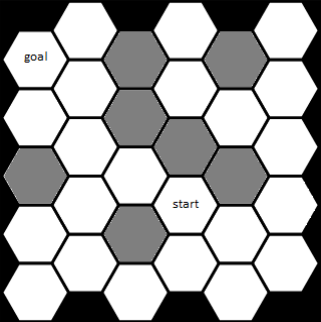
\includegraphics[scale=.75]{hextiles.png}  
\end{center}
\bigskip

\noindent\textbf{Part a:} What is the minimum number of cells that the shortest path first algorithm needs to expand in the grid shown above before finding a path to the goal (and why)?
\bigskip

\noindent\textbf{Answer:} Below is the figure with cells labeled in the alphabetical order they were first discovered:
\begin{center}
  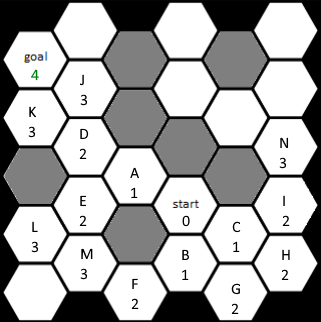
\includegraphics[scale=.75]{hextiles2a.png}  
\end{center}

Note that the order cells are discovered is starting with the cell directly above and moving counterclockwise. Also note that the way ties are broken is to favor cells discovered first.

We can see that 11 cells had to be expanded, namely $\{start,A,B,C,D,E,F,G,H,I,J\}$, for a path to the goal cell to be found.

% finally be added to the set of completed cells (of course, a path was found after 11 expansions but the algorithm dictates we explore the next 4 cells to be sure no better path exists before we add the goal cell to the completed set).

Since our method of discovery and tie-breaking gets us to the goal the fastest, 11 is the minimum number of expansions an SPF implementation could make.
\bigskip

\newpage
\noindent\textbf{Part b:} Define an admissible heuristic for this problem. Show that this heuristic is admissible.
\bigskip

\noindent\textbf{Answer:} Let us define a metric, analogous to the manhattan distance, on the hex grid called the `hex distance.' The hex distance is just the shortest distance between two hex cells (disregarding obstructions):
\begin{center}
  \includegraphics[scale=.75]{hextilesdist.png}  
\end{center}

Now recall that for a heuristic $h(x)$ to be admissable it must be less than or equal to the true cost, which in this case is the length of the shortest path to the goal. You'll note that since the hex distance is the minimum distance to the goal (without obstructions), it will always be less than or equal to the true distance (with obstructions) to the goal. As such, the hex distance can serve as a valid heuristic $h(x)$:
$$h(x)=\text{hex distance from $x$ to goal}$$
\medskip

\noindent\textbf{Part c:} What is the minimum number of cells that A* with your heuristic needs to expand in the given grid before finding a path to the goal?
\bigskip

\noindent\textbf{Answer:} Below is a figure analogous to the one in part a, but this time each cell has a value that is the sum of its distance from the start goal \textit{and} its heuristic (also note that despite some nodes now being undiscovered, the nodes are still in alphebetical order of discovery):
\begin{center}
  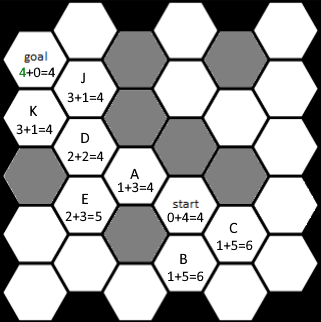
\includegraphics[scale=.75]{hextiles3.png}
\end{center}

Equipped with this heuristic, our A* implementation makes only 4 expansions before the goal is found. These are at $\{start,A,D,J\}$.

% Of course, like before, a path is found after 4 expansions but the algorithm dictates we expand the next cell to be sure it is the shortest path.

\newpage
\subsection*{Question 3}
The table below contains a list of Lord of the Rings characters along with their character class and a set of other attributes.
\begin{center}
  \begin{tabular}{ c | c | c | c | c | c }
    \toprule
    & & \multicolumn{4}{c}{\textbf{Attributes}} \\ \hline
    \textbf{Character} & \textbf{Class} & \textbf{Weapon} & \textbf{Height} & \textbf{Armor} & \textbf{Age} \\ \hline
    Gandalf & Wizard & Staff & Tall & No & $>$1000 \\ \hline
    Bilbo & Hobbit & Dagger & Short & No & 100-1000 \\ \hline
    Legolas & Elf & Bow & Tall & No & $>$1000 \\ \hline
    Saruman & Wizard & Staff & Tall & No & $>$1000 \\ \hline
    Elrond & Elf & Sword & Tall & Yes & $>$1000 \\ \hline
    Frodo & Hobbit & Dagger & Short & Yes & $<$100 \\ \hline
    Aragon & Human & Sword & Tall & No & $<$100 \\ \hline
    Gimli & Dwarf & Ax & Short & Yes & 100-1000 \\ \hline
    Thorin & Dwarf & Sword & Short & Yes & 100-1000 \\ \hline
    Boromir & Human & Sword & Tall & Yes & $<$100 \\ \hline
    Faramir & Human & Bow & Tall & No & $<$100 \\
    \bottomrule
  \end{tabular}
\end{center}
\bigskip


\noindent\textbf{Part a:} What is the information gain of dividing this set on the Weapon attribute.
\bigskip

\noindent\textbf{Answer:} 
First we compute the entropy $E(S)$ of the set of characters $S$ with respect to their classes:
\begin{align*}
  E(S)&=\overbrace{-\frac{2}{11}\log_2\left(\frac{2}{11}\right)}^{\text{Wizard}}
  \overbrace{-\frac{2}{11}\log_2\left(\frac{2}{11}\right)}^{\text{Hobbit}}
  \overbrace{-\frac{2}{11}\log_2\left(\frac{2}{11}\right)}^{\text{Elf}}
  \overbrace{-\frac{3}{11}\log_2\left(\frac{3}{11}\right)}^{\text{Human}}
  \overbrace{-\frac{2}{11}\log_2\left(\frac{2}{11}\right)}^{\text{Dwarf}}\\
  &\approx0.447169+0.447169+0.447169+0.511219+0.447169\\
  &\approx2.299896
\end{align*}

Now we partition $S$ with respect to the Weapon class and compute each subset $S_i$'s entropy with respect to class:
\begin{align*}
  E(S_{\text{Staff}})&=\overbrace{-\frac{2}{2}\log_2\left(\frac{2}{2}\right)}^{\text{Wizard}}=0\\
  E(S_{\text{Dagger}})&=\overbrace{-\frac{2}{2}\log_2\left(\frac{2}{2}\right)}^{\text{Hobbit}}=0\\
  E(S_{\text{Bow}})&=\overbrace{-\frac{1}{2}\log_2\left(\frac{1}{2}\right)}^{\text{Elf}}
  \overbrace{-\frac{1}{2}\log_2\left(\frac{1}{2}\right)}^{\text{Human}}=0.5+0.5=1\\
  E(S_{\text{Sword}})&=\overbrace{-\frac{1}{4}\log_2\left(\frac{1}{4}\right)}^{\text{Elf}}
  \overbrace{-\frac{2}{4}\log_2\left(\frac{2}{4}\right)}^{\text{Human}}
  \overbrace{-\frac{1}{4}\log_2\left(\frac{1}{4}\right)}^{\text{Dwarf}}=0.5+0.5+0.5=1.5\\
  E(S_{\text{Ax}})&=\overbrace{-\frac{1}{1}\log_2\left(\frac{1}{1}\right)}^{\text{Dwarf}}=0
\end{align*}
\newpage

Now we compute the following sum:
\begin{align*}
  \sum_{i\in\text{Weapon}}|S_i|\cdot E(S_i)&=2\cdot0+2\cdot0+2\cdot1+4\cdot1.5+1\cdot0=8
\end{align*}

We can now compute the information gain of splitting $S$ on the Weapon attribute:
\begin{align*}
  \operatorname{Gain}(S,\text{Weapon})&=E(S)-\frac{1}{|S|}\sum_{i\in\text{Weapon}}|S_i|\cdot E(S_i)\\
  &\approx2.299896-\frac{8}{11}\\
  &\approx1.572623\text{ bits}
\end{align*}

\noindent\textbf{Part b:} Construct a decision tree using the ID3 algorithm that classifies the characters using the provided attributes.
\bigskip

\noindent\textbf{Answer:} Below is a decision tree that classifies the above charactres based on the given attributes.
\begin{center}
  \begin{forest}
    for tree={l sep+=.8cm,s sep+=.5cm,shape=rectangle, rounded corners,
        draw, align=center,
        top color=white, bottom color=white}
    [Weapon
      [\textbf{Wizard},edge label={node[midway,left]{Staff}} ]
      [\textbf{Hobbit},edge label={node[midway,midway]{Dagger}}]
      [Age,edge label={node[midway,right]{Bow}}
        [\textbf{Human},edge label={node[midway,left]{$<\!\!100$}}]
        [\textbf{Elf},edge label={node[midway,right]{$>\!\!1000$}}]
      ]
      [Age,edge label={node[midway,midway]{Sword}}
        [\textbf{Human},edge label={node[midway,left]{$<\!\!100$}}]
        [\textbf{Elf},edge label={node[midway,right]{$>\!\!1000$}}]
      ]
      [\textbf{Dwarf},edge label={node[midway,right]{Ax}}]
    ]  
  \end{forest}
\end{center}

% Below is the binary tree I made before the problem statement was changed...
% \begin{center}
%   \begin{forest}
%     for tree={l sep+=.8cm,s sep+=.5cm,shape=rectangle, rounded corners,
%         draw, align=center,
%         top color=white, bottom color=white}
%     [Short?
%       [Dagger?,edge label={node[midway,left]{$\checkmark$}} 
%         [\textbf{Hobbit},edge label={node[midway,left]{$\checkmark$}}]
%         [\textbf{Dwarf},edge label={node[midway,right]{$\times$}}]
%       ]
%       [$<$100?,edge label={node[midway,right]{$\times$}} 
%         [\textbf{Human},edge label={node[midway,left]{$\checkmark$}}]
%         [Staff?,edge label={node[midway,right]{$\times$}}
%           [\textbf{Wizard},edge label={node[midway,left]{$\checkmark$}}]
%           [\textbf{Elf},edge label={node[midway,right]{$\times$}}]
%         ]
%       ]
%     ]  
%   \end{forest}
% \end{center}

% used https://planetcalc.com/8443/ with this data:
% Weapon;Height;Armor;Age;Class
% Staff;Tall;No;>1000;Wizard
% Dagger;Short;No;100x1000;Hobbit
% Bow;Tall;No;1000;Elf
% Staff;Tall;No;1000;Wizard
% Sword;Tall;Yes;1000;Elf
% Dagger;Short;Yes;100;Hobbit
% Sword;Tall;No;100;Human
% Ax;Short;Yes;100x1000;Dwarf
% Sword;Short;Yes;100x1000;Dwarf
% Sword;Tall;Yes;100;Human
% Bow;Tall;No;100;Human

\subsection*{Question 4}
Show that the following proposition is (or is not) an tautology:
$$((A\vee B)\wedge(\neg A\vee C)\wedge(B\vee D)\wedge(\neg C\vee E)\wedge(\neg D\vee E))\implies E$$

\noindent\textbf{Answer:} Consider the following counterexample with $A=C=D=E=F$ and $B=T$, where ($F=false$ and $T=true$):
\begin{align*}
&\,((A\vee B)\wedge(\neg A\vee C)\wedge(B\vee D)\wedge(\neg C\vee E)\wedge(\neg D\vee E))\implies E\\
\equiv &\,((F\vee T)\wedge(\neg F\vee F)\wedge(T\vee F)\wedge(\neg F\vee F)\wedge(\neg F\vee F))\implies F\tag{plug in truth values}\\
\equiv &\,((F\vee T)\wedge(T\vee F)\wedge(T\vee F)\wedge(T\vee F)\wedge(T\vee F))\implies F\\
\equiv &\,(T\wedge T\wedge T\wedge T\wedge T)\implies F\\
\equiv &\,T\implies F\\
\equiv &\,F
\end{align*}

As we can see, this particular setting of the variables makes the above proposition false, and so it is not a tautology.

\newpage
\subsection*{Question 5}
Consider the following Bayesian network, where $A,B,C,D$, and $E$ are all booleans:
\begin{center}
  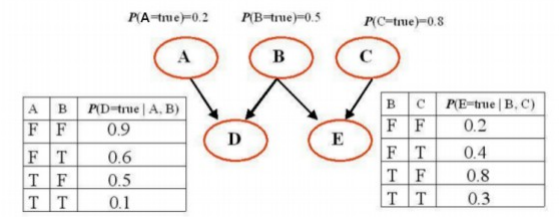
\includegraphics[scale=.75]{baysiannet.png}  
\end{center}
\bigskip

\noindent\textbf{Part a:} What is the probability that all five of these variables are simultaneously true?
\bigskip

\noindent\textbf{Answer:} The desired probability is given by:
\begin{align*}
  P(ABCDE)&=P(A)P(B)P(C)P(D|AB)P(E|BC)\\
  &=(.2)(.5)(.8)(.1)(.3)\\
  &=.0024
\end{align*}

\noindent\textbf{Part b:} What is the probability that all five of these variables are simultaneously false?
\bigskip

\noindent\textbf{Answer:} The desired probability is given by:
\begin{align*}
  P(A^\complement B^\complement C^\complement D^\complement E^\complement)&=P(A^\complement)P(B^\complement)P(C^\complement)P(D^\complement|A^\complement B^\complement)P(E^\complement|B^\complement C^\complement)\\
  &=(1-P(A))(1-P(B))(1-P(C))(1-P(D|A^\complement B^\complement))(1-P(E|B^\complement C^\complement))\\
  &=(1-.2)(1-.5)(1-.8)(1-.9)(1-.2)\\
  &=(.8)(.5)(.2)(.1)(.8)\\
  &=.0064
\end{align*}

\noindent\textbf{Part c:} What is the probability that $A$ is false given that the four other variables are all known to be true?
\smallskip

\noindent\textbf{Answer:} First let us compute the following joint probability:
\begin{align*}
  P(A^\complement BCDE)&=P(A^\complement)P(B)P(C)P(D|A^\complement B)P(E|BC)\\
  &=(.8)(.5)(.8)(.6)(.3)\\
  &=0.0576
\end{align*}

We can now use this to compute our desired probability:
\begin{align*}
  P(A^\complement|BCDE)&=\frac{P(A^\complement BCDE)}{P(BCDE)}\tag{Bayes' Theorem}\\
  &=\frac{P(A^\complement BCDE)}{P(ABCDE)+P(A^\complement BCDE)}\tag{law of total probability}\\
  &=\frac{P(A^\complement BCDE)}{.0024+P(A^\complement BCDE)}\tag{part a}\\
  &=\frac{0.0576}{.0024+0.0576}\tag{above calculation}\\
  &= 0.96
\end{align*}
% \begin{align*}
%   P(A^\complement|BCDE)&=\frac{P(A^\complement BCDE)}{P(BCDE)}\\
%   &=\frac{P(A^\complement)P(B)P(C)P(D|A^\complement B)P(E|BC)}{P(B)P(C)(P(D|AB)+P(D|A^\complement B))P(E|BC)}\\
%   &=\frac{(.8)(.5)(.8)(.6)(.3)}{(.5)(.8)(.1+.6)(.3)}\\
%   &=\frac{0.0576}{0.084}\\
%   &\approx 0.685714286
% \end{align*}
\end{document}